\documentclass[10pt,a4paper,headinclude,footinclude,hidelinks]{scrreprt} % KOMA-Script
\usepackage[italian]{babel}
\usepackage[utf8]{inputenc}
\usepackage[T1]{fontenc}
\usepackage{graphicx}
\usepackage{amsfonts}
\usepackage[]{../../classicthesis} % nochapters
\pagestyle{scrheadings}
\setcounter{tocdepth}{2}

\begin{document}
    \title{\rmfamily\normalfont\spacedallcaps{Progettazione}}
    \author{\spacedlowsmallcaps{Nicola Moretto (matr. 578258)}}
    \date{\today}
    
    \maketitle
    
    \begin{abstract}
        \noindent Il documento riporta le informazioni di progettazione riguardanti l'interfaccia grafica per la visualizzazione e la navigazione dei contenuti.
    \end{abstract}
    
	\begin{table}[ht]
	\centering
	\begin{tabular}{|c|c|l|}
	\hline
	\textsc{Versione} & \textsc{Data} & \textsc{Modifiche} \\ \hline
	0.1 & 15-10-2012 & Stesura iniziale del documento. \\ \hline
	0.2 & 17-10-2012 & Redatto il capitolo \ref{ch:stage:design:architettura}. \\ \hline
	0.3 & 18-10-2012 & Redatte le sezioni \ref{sec:stage:design:sistema:model.filter}, \ref{sec:stage:design:sistema:view.filter} e \ref{sec:stage:design:sistema:view.search}. \\ \hline
	0.4 & 19-10-2012 & Redatti i capitoli \ref{ch:stage:design:model} e \ref{ch:stage:design:view}. \\ \hline
	0.5 & 20-10-2012 & Revisione del documento. \\ \hline
	1.0 & 20-10-2012 & Pubblicazione della prima versione. \\ \hline
	1.1 & 22-10-2012 & Aggiunta la sezione \ref{sec:stage:design:sistema:model.provider}. \\ \hline
	1.2 & 23-10-2012 & Aggiornamento del capitolo \ref{ch:stage:design:model}. \\ \hline
	1.3 & 24-10-2012 & Aggiornamento del capitolo \ref{ch:stage:design:model}. \\ \hline
	\end{tabular}
	\caption{Registro delle modifiche}
	\label{tab:stage:wp:workload}
	\end{table}

	\tableofcontents

	%----------
	% CAPITOLO
	%----------
	\chapter{Introduzione}
	\label{ch:stage:design:intro}

%	\section{Obiettivi}
%	\begin{itemize}
%	\item aggiunta, rimozione o aggiornamento (motore di ricerca) di nuovi ambiti di ricerca;
%	\end{itemize}

%	\section{To do}
%	\begin{itemize}
%	\item Aggiungere la lista di informazioni essenziali e aggiuntive di un contenuto nei requisiti.
%	\end{itemize}

	\section{Riferimenti informativi}
	\begin{itemize}
	\item Analisi dei requisiti (\textit{analisi\_dei\_requisiti\_1.0} allegata alla presente documentazione);
	\item Sistema di classificazione (\textit{sistema\_di\_classificazione\_2.0} allegato alla presente documentazione).
	\end{itemize}

	%----------
	% CAPITOLO
	%----------
	\chapter{Architettura}
	\label{ch:stage:design:architettura}

	\section{Architettura generale}
	\label{sec:stage:design:architettura:mvc}
	L'architettura del sistema software rispecchia il design pattern architetturale MVC, che prevede e garantisce la separazione delle tre componenti fondamentali del sistema:
	\begin{description}
	\item[Model] Racchiude i dati e le informazioni dell'applicazione e definisce le modalità di accesso e fruizione degli stessi da parte delle altre componenti (\textit{Controller} e \textit{View}).
 	\item[View] Rappresenta l'interfaccia grafica mediante la quale vengono visualizzate le informazioni e i dati conservati nel \textit{Model} e l'utente può interagire con il sistema. La rilevazione dell'avvenuta interazione dell'utente è responsabilità di tale componente, mentre la gestione della reazione è demandata al \textit{Controller}.
	\item[Controller] Incorpora la logica di controllo dell'applicazione, inizializzando il sistema e traducendo l'interazione dell'utente con l'interfaccia grafica (\textit{View}) in operazioni sui dati (\textit{Model}).
	\end{description}

	\section{Componenti architetturali}
	\label{sec:stage:design:mvc}

	\subsection{Componente Model}
	\label{sec:stage:design:mvc:model}
	La componente \textit{model} conserva tutte i tipi di informazioni connessi alla ricerca:
	\begin{itemize}
	\item gli ambiti (etichette, frasi);
	\item i criteri (termini di ricerca, entità);
	\item i filtri (argomento, data di pubblicazione, emozioni, \ldots);
	\item i risultati (contenuti informativi).
	\end{itemize}

	\subsection{Componente View}
	\label{sec:stage:design:mvc:view}
	La componente \textit{view} rappresenta l'interfaccia grafica mediante la quale l'utente interagisce con il sistema per effettuare una ricerca, raffinarne i criteri o consultarne i risultati.

	\paragraph{Livelli}
	Essa è organizzata in quattro livelli (o strati) distinti, che includono rispettivamente:
	\begin{itemize}
	\item gli strumenti e le informazioni connesse alla ricerca (barra di ricerca, etichette, entità, \ldots);
	\item i filtri di ricerca;
	\item i risultati della ricerca (proprietà e relazioni dei contenuti informativi;
	\item la cronologia (organizzazione temporale dei contenuti).
	\end{itemize}

	\subsection{Componente Controller}
	\label{sec:stage:design:mvc:controller}
	La componente \textit{controller} gestisce l'interazione dell'utente con l'interfaccia grafica e le operazioni connesse alla ricerca e alla visualizzazione dei contenuti informativi, tra cui:
	\begin{itemize}
	\item la configurazione dei criteri di ricerca (selezione di un'accezione di un'etichetta, gestione delle entità);
	\item il reperimento dei contenuti informativi corrispondenti ai criteri di ricerca;
	\item la gestione dei filtri di ricerca;
	\item l'aggiornamento dei risultati di ricerca visualizzati a fronte di modifiche alle entità e ai filtri di ricerca;
	\item \ldots
	\end{itemize}

	%----------
	% CAPITOLO
	%----------
	\chapter{Componente Model}
	\label{ch:stage:design:model}

	\begin{figure}[ht]
		\begin{center}
	    	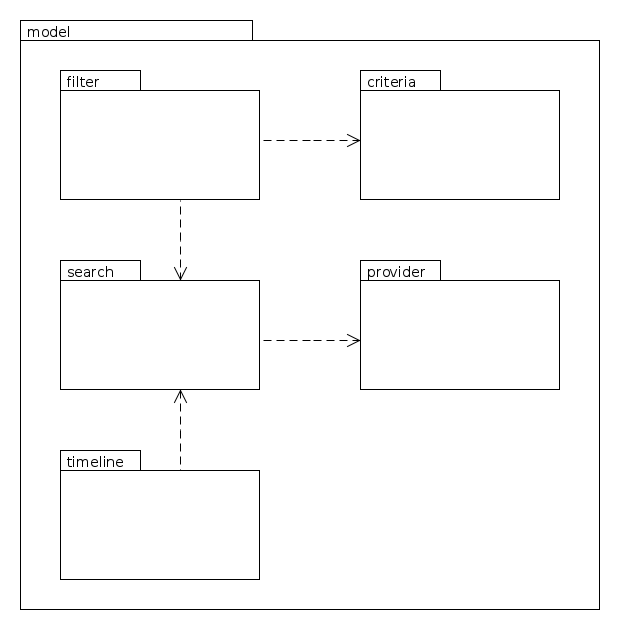
\includegraphics[width=10cm]{package/model.png}
			\label{gfx:package:model}
			\caption{Diagramma del package \textit{model}}
		\end{center}
	\end{figure}

	Questo capitolo illustra i componenti del \textit{Model}, per ciascuno dei quali è indicato il nome della classe accompagnata da un'identificazione sintetica, separati dal carattere '|' (separatore verticale).

	% SECTION
	\section{Package model}
	\label{sec:stage:design:sistema:model}

	\subsection[Entity]{Entity | Entità del dominio}
	\label{sec:stage:design:sistema:model:entity}
	La classe modella le entità del dominio della piattaforma, a ciascuna delle quali è associata un'etichetta - in una specifica accezione - che la identifica univocamente nell'ambito della piattaforma (\textit{\nameref{sec:stage:design:sistema:model:label}}).

	\subsection[Label]{Label | Etichetta del dizionario}
	\label{sec:stage:design:sistema:model:label}
	La classe modella le etichette del dizionario della piattaforma, ciascuna delle quali può possedere molteplici accezioni (\textit{\nameref{sec:stage:design:sistema:model:meaning}}).

	\subsection[Meaning]{Meaning | Accezione di un'etichetta}
	\label{sec:stage:design:sistema:model:meaning}
	La classe modella un'accezione di un'etichetta (\textit{\nameref{sec:stage:design:sistema:model:label}}), cui è associata un entità del dominio (\textit{\nameref{sec:stage:design:sistema:model:entity}}).

	% SECTION
	\section{Package model.content}
	\label{sec:stage:design:sistema:model.content}

	\subsection[Content]{Content | Contenuto informativo}
	\label{sec:stage:design:sistema:model.content:content}
	La classe astratta rappresenta un generico contenuto informativo pubblicato dagli utenti nella piattaforma, caratterizzato delle seguenti proprietà:
	\begin{itemize}
	\item autore (\textit{\nameref{sec:stage:design:sistema:model.criteria:user}});
	\item data di pubblicazione (\textit{\nameref{sec:stage:design:sistema:model.criteria:publication-date}});
	\item titolo.
	\end{itemize}

	\subsection[ContentManager]{ContentManager | Gestione dei contenuti}
	\label{sec:stage:design:sistema:model.content:content-manager}
	Interfaccia del package \textit{model.content} per la gestione dei contenuti (\textit{\nameref{sec:stage:design:sistema:model.content:content}}) istanziati.

	\subsection[Answer]{Answer | Risposta}
	\label{sec:stage:design:sistema:model.content:answer}

	\paragraph{Dipendenze} Estende la classe \textit{\nameref{sec:stage:design:sistema:model.content:content}}.

	\subsection[Event]{Event | Evento}
	\label{sec:stage:design:sistema:model.content:event}

	\paragraph{Dipendenze} Estende la classe \textit{\nameref{sec:stage:design:sistema:model.content:content}}.

	\subsection[Message]{Message | Comunicazione privata}
	\label{sec:stage:design:sistema:model.content:message}

	\paragraph{Dipendenze} Estende la classe \textit{\nameref{sec:stage:design:sistema:model.content:content}}.

	\subsection[Question]{Question | Domanda}
	\label{sec:stage:design:sistema:model.content:question}

	\paragraph{Dipendenze} Estende la classe \textit{\nameref{sec:stage:design:sistema:model.content:content}}.

	\subsection[Review]{Review | Recensione}
	\label{sec:stage:design:sistema:model.content:review}

	\paragraph{Dipendenze} Estende la classe \textit{\nameref{sec:stage:design:sistema:model.content:content}}.

	\subsection[Talk]{Talk | Discorso}
	\label{sec:stage:design:sistema:model.content:talk}

	\paragraph{Dipendenze} Estende la classe \textit{\nameref{sec:stage:design:sistema:model.content:content}}.

	\subsection[Thought]{Thought | Pensiero}
	\label{sec:stage:design:sistema:model.content:thought}
	
	\paragraph{Dipendenze} Estende la classe \textit{\nameref{sec:stage:design:sistema:model.content:content}}.

	% SECTION
	\section{Package model.criteria}
	\label{sec:stage:design:sistema:model.criteria}
	Ciascun contenuto può essere classificato in accordo a differenti criteri, ciascuno dei quali ne prende in esame una differente proprietà, come l'autore, la data di pubblicazione, il tipo, le emozioni associate, \ldots .

	Ciascuna proprietà può essere propria del contenuto o funzionale al contesto di ricerca (attinenza, \ldots).

	\subsection[Criterion]{Criterion | Criterio di classificazione}
	\label{sec:stage:design:sistema:model.criteria:criteria}
	Interfaccia dei (tipi di) criteri di classificazione.

	\subsection[ListCriterion]{ListCriterion | Criterio basato su una lista di valori}
	\label{sec:stage:design:sistema:model.criteria:list-criterion}
	La classe \textit{\nameref{sec:stage:design:sistema:model.criteria:list-criterion}} viene utilizzata in combinazione con un filtro \textit{\nameref{sec:stage:design:sistema:model.filter:list-filter}}, fornendo i valori e i parametri di configurazione iniziale.

	\subsection[RangeCriterion]{RangeCriterion | Criterio basati su un intervallo di valori}
	\label{sec:stage:design:sistema:model.criteria:range-criterion}
	La classe \textit{\nameref{sec:stage:design:sistema:model.criteria:range-criterion}} viene utilizzata in combinazione con un filtro \textit{\nameref{sec:stage:design:sistema:model.filter:range-filter}}, fornendo i valori e i parametri di configurazione iniziale.

	\subsection[SwitchCriterion]{SwitchCriterion | Criterio a doppio stato}
	\label{sec:stage:design:sistema:model.criteria:switch-criterion}
	La classe \textit{\nameref{sec:stage:design:sistema:model.criteria:switch-criterion}} viene utilizzata in combinazione con un filtro \textit{\nameref{sec:stage:design:sistema:model.filter:switch-filter}}, fornendo i valori e i parametri di configurazione iniziale.

	\subsection[ValueCriterion]{ValueCriterion | Filtro basato su una soglia di valore}
	\label{sec:stage:design:sistema:model.criteria:value-criterion}
	La classe \textit{\nameref{sec:stage:design:sistema:model.criteria:value-criterion}} viene utilizzata in combinazione con un filtro \textit{\nameref{sec:stage:design:sistema:model.filter:value-filter}}, fornendo i valori e i parametri di configurazione iniziale.

	\subsection[CriterionData]{CriterionData | Sorgente dati per un criterio di classificazione}
	\label{sec:stage:design:sistema:model.criteria:criterion-data}
	Classe astratta dei componenti che forniscono liste di valori per i criteri di classificazione.
	% Campo dati statico: riferimento ai risultati di ricerca
	% Sottoclassi: metodo statico che restituisce i valori richiesti (lista, min, max, ...)
	% Sottoclasse lista con valori predefiniti: campo dati statico con lista di valori dello stesso tipo della classe

	\subsection[Emotion]{Emotion | Emozione}
	\label{sec:stage:design:sistema:model.criteria:emotion}

	\subsection[Intention]{Intention | Intenzione}
	\label{sec:stage:design:sistema:model.criteria:intention}

	\subsection[PublicationDate]{PublicationDate | Data di pubblicazione}
	\label{sec:stage:design:sistema:model.criteria:publication-date}

	\subsection[Rating]{Rating | Giudizio}
	\label{sec:stage:design:sistema:model.criteria:rating}

	\subsection[Relevance]{Relevance | Attinenza}
	\label{sec:stage:design:sistema:model.criteria:relevance}

	\subsection[Topic]{Topic | Argomento}
	\label{sec:stage:design:sistema:model.criteria:topic}

	\subsection[Type]{Type | Tipo di contenuto}
	\label{sec:stage:design:sistema:model.criteria:type}

	\subsection[User]{User | Utente}
	\label{sec:stage:design:sistema:model.criteria:user}
	La classe rappresenta un utente della piattaforma, potenziale autore di contenuti.

	% SECTION	
	\section{Package model.filter}
	\label{sec:stage:design:sistema:model.filter}
	Ciascun filtro è associato ad una proprietà dei risultati di ricerca (\textit{\nameref{sec:stage:design:sistema:model.criteria:criteria}}) e partiziona automaticamente l'insieme dei possibili valori in due sottoinsiemi: ammessi o bloccati. Nella configurazione iniziale, tutti i valori possibili di una proprietà sono ammessi, mentre l'utente può intervenire secondo modalità differenti per alterare tale partizionamento (vedi sezione \ref{sec:stage:design:sistema:view.filter}).
	
	Il valore che ciascun contenuto (da intendersi come risultato di una ricerca) ha rispetto ad una proprietà associata ad un filtro può quindi appartenere ad uno dei due sottoinsiemi: il contenuto viene mostrato solo se tutti i valori delle proprietà in questione risultano ammessi.

	\subsection[Filter]{Filter | Filtro di ricerca}
	\label{sec:stage:design:sistema:model.filter:filter}
	Tale componente rappresenta l'interfaccia dei filtri per il raffinamento dei risultati di una ricerca e viene implementata dalle classi che modellano le tipologie standard di filtri di ricerca (\textit{\nameref{sec:stage:design:sistema:model.filter:list-filter}}, \textit{\nameref{sec:stage:design:sistema:model.filter:range-filter}}, \textit{\nameref{sec:stage:design:sistema:model.filter:switch-filter}} e \textit{\nameref{sec:stage:design:sistema:model.filter:value-filter}}).
	
	Ciascuna istanza di una sottoclasse concreta è associata ai risultati di una ricerca specifica (\textit{\nameref{sec:stage:design:sistema:model.search:search-result}}), su cui si applica il filtro corrispondente.

	\subsection[FilterManager]{FilterManager | Gestione dei filtri}
	\label{sec:stage:design:sistema:model.filter:filter-manager}
	Tale componente rappresenta l'interfaccia del package \textit{model.filter}, utile a esporre le funzionalità per l'istanziazione e la gestione dei filtri.
	%\paragraph{Design Pattern:} Facade, Singleton

	\subsection[ListFilter]{ListFilter | Filtro a lista di valori}
	\label{sec:stage:design:sistema:model.filter:list-filter}
	Il componente modella un filtro basato su una lista di possibili valori, ciascuno dei quali può essere autorizzato o bloccato dall'utente.

	\paragraph{Dipendenze:} Ogni istanza della classe \textit{\nameref{sec:stage:design:sistema:model.filter:list-filter}} è associata ad un criterio \textit{\nameref{sec:stage:design:sistema:model.criteria:list-criterion}}.

	\subsection[RangeFilter]{RangeFilter | Filtro ad intervallo di valori}
	\label{sec:stage:design:sistema:model.filter:range-filter}
	Il componente modella un filtro basato su un intervallo di valori ordinati (numeri, date, \ldots). Siano $inf$ e $sup$ rispettivamente l'estremo inferiore e superiore dell'intervallo: risultano dunque ammessi tutti e soli i valori $v$ tali che $v \in \left[inf,sup\right]$.

	All'utente è consentito scegliere i valori desiderati di $inf$ e $sup$ tali che:
	\begin{itemize}
	\item $sup$ sia un valore valido;
	\item $inf$ sia un valore valido;
	\item $inf \leq sup$;
	\item se è definito un valore attuale $current$, allora deve valere $min \leq current \leq max$.
	\end{itemize}

	Se l'insieme dei valori ordinati prevede un minimo $min$ e/o un massimo $max$ si aggiungono le seguenti condizioni:
	\begin{itemize}
	\item $sup \leq max$;
	\item $inf \geq min$.
	\end{itemize}

	\paragraph{Dipendenze:} Ogni istanza della classe \textit{\nameref{sec:stage:design:sistema:model.filter:range-filter}} è associata ad un criterio \textit{\nameref{sec:stage:design:sistema:model.criteria:range-criterion}}.

	\subsection[SwitchFilter]{SwitchFilter | Filtro a doppio stato}
	\label{sec:stage:design:sistema:model.filter:switch-filter}
	Il componente modella un filtro il cui partizionamento è predefinito e invariabile e che l'utente può solamente abilitare o disattivare.

	\paragraph{Dipendenze:} Ogni istanza della classe \textit{\nameref{sec:stage:design:sistema:model.filter:switch-filter}} è associata ad un criterio \textit{\nameref{sec:stage:design:sistema:model.criteria:switch-criterion}}.

	\subsection[ValueFilter]{ValueFilter | Filtro a soglia di valore}
	\label{sec:stage:design:sistema:model.filter:value-filter}
	Il componente modella un filtro basato su una soglia di valore. Sia $value$ il valore scelto: in tal caso risultano ammessi tutti e soli i valori $x$ validi tali che $x \geq value$.

	Se l'insieme prevede un minimo $min$ e/o un massimo $max$ dev'essere soddisfatta anche la condizione $min \leq x \leq max$.

	\paragraph{Dipendenze:} Ogni istanza della classe \textit{\nameref{sec:stage:design:sistema:model.filter:value-filter}} è associata ad un criterio \textit{\nameref{sec:stage:design:sistema:model.criteria:value-criterion}}.

	% SECTION	
	\section{Package model.provider}
	\label{sec:stage:design:sistema:model.provider}
	Le classi del package \textit{model.provider} forniscono le funzionalità necessarie ad interrogare la base di dati per reperire i contenuti informativi corrispondenti ai criteri di ricerca immessi e all'ambito specificato.

	Dal momento che tali operazioni verranno affidate a componenti terze, tuttora oggetto di analisi e valutazione, le scelte progettuali illustrate di seguito tengono conto di tale incertezza e sono pertanto da considerarsi non esaustive o definitive.

	\subsection[Provider]{Provider | Motore di ricerca}
	\label{sec:stage:design:sistema:model.search:search-provider}
	La componente rappresenta l'interfaccia standard implementata dai fornitori di ricerca (\textit{\nameref{sec:stage:design:sistema:model.search:tag-provider}}, \textit{\nameref{sec:stage:design:sistema:model.search:full-text-provider}}).

	\subsection[ProviderRegistry]{ProviderRegistry | Gestione dei fornitori di ricerca}
	\label{sec:stage:design:sistema:model.search:provider-registry}
	La componente gestisce le istanze delle classi \textit{\nameref{sec:stage:design:sistema:model.search:tag-provider}} e \textit{\nameref{sec:stage:design:sistema:model.search:full-text-provider}}.

	\subsection[LabelProvider]{LabelProvider | Ricerca delle etichette}
	\label{sec:stage:design:sistema:model.search:tag-provider}
	La classe fornisce le funzionalità necessaria a cercare dei termini di ricerca tra le etichette assegnate ai contenuti, considerandone le specifiche accezioni.

	\paragraph{Dipendenze} Implementa l'interfaccia \textit{\nameref{sec:stage:design:sistema:model.search:search-provider}} e le sue istanze vengono gestite da \textit{\nameref{sec:stage:design:sistema:model.search:provider-registry}}.

	\subsection[FullTextProvider]{FullTextProvider | Ricerca dei contenuti informativi}
	\label{sec:stage:design:sistema:model.search:full-text-provider}
	La classe permette di cercare la presenza dei termini di ricerca nel titolo, nel corpo o in altri campi di un contenuto informativo.

	\paragraph{Dipendenze} Implementa l'interfaccia \textit{\nameref{sec:stage:design:sistema:model.search:search-provider}} e le sue istanze vengono gestite da \textit{\nameref{sec:stage:design:sistema:model.search:provider-registry}}.

	% SECTION	
	\section{Package model.search}
	\label{sec:stage:design:sistema:model.search}

	\subsection[SearchEntityList]{SearchEntityList | Lista delle entità cercate}
	\label{sec:stage:design:sistema:model.search:search-entity-list}

	\subsection[SearchManager]{SearchManager | Gestione della ricerca}
	\label{sec:stage:design:sistema:model.search:search-manager}

	%\paragraph{Design Pattern} Facade

	\subsection[SearchQuery]{SearchQuery | Query di ricerca}
	\label{sec:stage:design:sistema:model.search:search-query}
	Tale componente modella la query di ricerca, ossia la stringa inserita dall'utente nella barra di ricerca (\textit{\nameref{sec:stage:design:sistema:view.search:search-bar}}) e contenente una lista di termini o espressioni separati da virgola.

	La classe fornisce i metodi per effettuare l'analisi sintattica della stringa al fine di estrapolare i termini (\textit{\nameref{sec:stage:design:sistema:model.search:search-term}}) da cercare e stabilire quali di essi siano etichette o frasi.

	\paragraph{Dipendenze} A ciascuna istanza della classe sono associati dei termini di ricerca (\textit{\nameref{sec:stage:design:sistema:model.search:search-term}}).

	\subsection[SearchResult]{SearchResult | Risultati della ricerca}
	\label{sec:stage:design:sistema:model.search:search-result}

	\paragraph{Dipendenze} Ciascuna istanza della classe gestisce un insieme di contenuti (\textit{\nameref{sec:stage:design:sistema:model.content:content}}) corrispondenti ai criteri di ricerca.

	\subsection[SearchScope]{SearchScope | Ambito di ricerca}
	\label{sec:stage:design:sistema:model.search:search-scope}
	La classe rappresenta il generico ambito di ricerca, che l'utente può selezionare mediante il corrispondente selettore (\textit{\nameref{sec:stage:design:sistema:view.search:search-scope-selector}}).

	\subsection[SearchTerm]{SearchTerm | Termine di ricerca}
	\label{sec:stage:design:sistema:model.search:search-term}
	La componente rappresenta un'interfaccia comune a tutti i tipi di termini di ricerca, ossia frasi e etichette.

	Ciascun termine di ricerca viene memorizzato all'interno di un'istanza di \textit{\nameref{sec:stage:design:sistema:model.search:search-query}} e viene passato al \textit{SearchManager} per consentire l'esecuzione della ricerca.

	% SECTION	
	\section{Package model.timeline}
	\label{sec:stage:design:sistema:model.timeline}

	\subsection[Timeline]{Timeline | Linea del tempo}
	\label{sec:stage:design:sistema:model.timeline:timeline}

	%----------
	% CAPITOLO
	%----------
	\chapter{Componente View}
	\label{ch:stage:design:view}

	\begin{figure}[ht]
		\begin{center}
	    	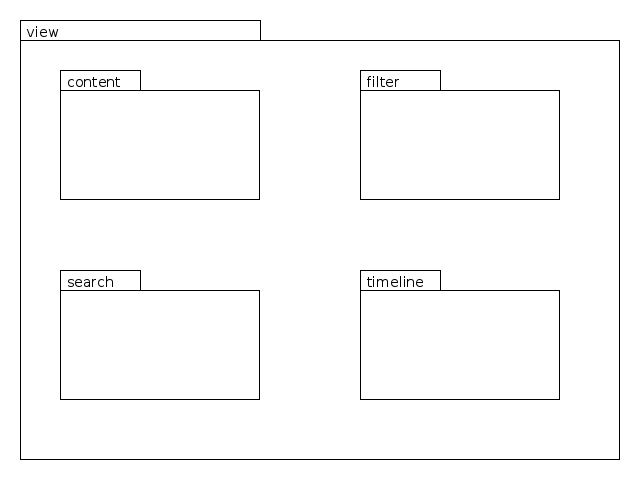
\includegraphics[width=10cm]{package/view.png}
			\label{gfx:package:view}
			\caption{Diagramma del package \textit{view}}
		\end{center}
	\end{figure}

	Questo capitolo illustra i componenti del \textit{View}, per ciascuno dei quali è indicato il nome della classe accompagnata da un'identificazione sintetica, separati dal carattere '|' (separatore verticale).

	% SECTION
	\section{Package view}
	\label{sec:stage:design:sistema:view}
	
	\subsection[MainWindow]{MainWindow | Finestra principale}
	La finestra principale rappresenta il contenitore all'interno del quale vengono inseriti e opportunamente collocati tutti gli elementi grafici dell'interfaccia, tra cui gli strumenti di ricerca, i filtri e i contenuti.

	% SECTION
	\section{Package view.content}
	\label{sec:stage:design:sistema:view.content}

	\subsection[ContentView]{ContentView | Contenuto informativo}
	Si tratta del componente grafico deputato a rappresentare graficamente un contenuto informativo, risultato di una ricerca effettuata dall'utente, e le relative informazioni, in formato grafico o testuale e distinte in essenziali o aggiuntive.

	Le informazioni essenziali\marginpar{Informazioni essenziali} sono utili per una immediato e preciso inquadramento del contenuto informativo da parte dell'utente al fine di stabilirne la rilevanza soggettiva.
	\begin{description}
	\item[Autore] L'autore del contenuto è l'utente (\textit{\nameref{sec:stage:design:sistema:model.criteria:user}}) che lo ha pubblicato all'interno della piattaforma e viene rappresentato testualmente mediante il suo \textit{nome utente} o \textit{proprio}.
	\item[Attinenza] Il grado di attinenza di un contenuto rispetto ai criteri di ricerca corrisponde - in percentuale - al rapporto tra le entità assegnate e quelle cercate. Tale informazione viene rappresentata graficamente variando proporzionalmente la \textit{dimensione} dell'elemento grafico.
	\item[Data di pubblicazione] La data di pubblicazione del contenuto viene indicata testualmente.
	\item[Tipo] Il tipo di contenuto (\textit{\nameref{sec:stage:design:sistema:model.content:content}}) viene rappresentato graficamente mediante la forma\footnote{Le forme utilizzate sono elementari per garantire l'immediata riconoscibilità da parte di qualsiasi tipo di utente, evitando l'impiego di forme potenzialmente ambigue o ignote a seconda del suo profilo sociale, culturale, geografico, \ldots} specifica dell'elemento grafico e può essere:
	\item[Titolo] Il titolo assegnato al contenuto rappresenta un'informazione chiave e viene rappresentata in formato testuale.
	\end{description}

	Le informazioni aggiuntive\marginpar{informazioni aggiuntive} forniscono all'utente dettagli utili per approfondire l'esame di un contenuto.
	\begin{description}
	\item[Argomento] Ciascun contenuto può riferirsi al più ad un argomento, rappresentabile in maniera grafica (colore o simbolo) o testuale.
	\item[Emozioni] A ciascun contenuto possono essere associate diverse emozioni, che esprimono lo stato d'animo dell'autore al momento della sua redazione o pubblicazione. La lista delle emozioni associate ad un contenuto viene visualizzata in formato testuale.
	\item[Entit\`a] A ciascun contenuto possono essere assegnate delle etichette, che riferiscono altrettante entità del dominio da visualizzare in formato testuale (mediante il rispettivo nome).
	\item[Intenzioni] A ciascun contenuto possono essere associate delle intenzioni, che possano fornire delle linee guida interpretative ai lettori. La lista delle intenzioni associate ad un contenuto viene visualizzata in formato testuale.
	\end{description}

	% SECTION
	\section{Package view.filter}
	\label{sec:stage:design:sistema:view.filter}

	\subsection[FilterContainer]{FilterContainer | Livello filtri}
	Il \textit{FilterContainer} raccoglie e mantiene separati in un livello distinto gli elementi grafici di tipo \textit{\nameref{sec:stage:design:sistema:view.filter:filter}}, che forniscono all'utente gli strumenti per impostare i filtri di ricerca.
	
	%\paragraph{Design pattern:} Facade, Singleton.

	\subsection[FilterView]{FilterView | Filtro di ricerca}
	\label{sec:stage:design:sistema:view.filter:filter}
	Si tratta dell'interfaccia delle componenti grafiche, che rappresentano le tipologie standard dei filtri per il raffinamento dei risultati di una ricerca, ossia (\textit{\nameref{sec:stage:design:sistema:view.filter:list-filter}}, \textit{\nameref{sec:stage:design:sistema:view.filter:range-filter}}, \textit{\nameref{sec:stage:design:sistema:view.filter:switch-filter}} e \textit{\nameref{sec:stage:design:sistema:view.filter:value-filter}}).

	\subsection[ListFilterView]{ListFilterView | Filtro con lista di valori}
	\label{sec:stage:design:sistema:view.filter:list-filter}
	Il componente grafico - associato alla classe \textit{\nameref{sec:stage:design:sistema:model.filter:list-filter}} - visualizza le liste dei valori ammissibili e bloccati e consente all'utente di:
	\begin{itemize}
	\item spostare un valore da una lista all'altra;
	\item azzerare il filtro, spostando automaticamente tutti i valori nella lista degli ammissibili.
	\end{itemize}

	\subsection[RangeFilterView]{RangeFilterView | Filtro con intervallo di valori}
	\label{sec:stage:design:sistema:view.filter:range-filter}
	Il componente grafico - associato alla classe \textit{\nameref{sec:stage:design:sistema:model.filter:range-filter}} - permette all'utente di specificare l'estremo inferiore e superiore dell'intervallo dei valori ammissibili secondo le regole definite nella suddetta classe.

	\subsection[SwitchFilterView]{SwitchFilterView | Filtro a doppio stato}
	\label{sec:stage:design:sistema:view.filter:switch-filter}
	Il componente grafico - associato alla classe \textit{\nameref{sec:stage:design:sistema:model.filter:switch-filter}} - consente di abilitare o disattivare il filtro corrispondente o di visualizzarne lo stato corrente.

	\subsection[ValueFilterView]{ValueFilterView | Filtro con soglia di valore}
	\label{sec:stage:design:sistema:view.filter:value-filter}
	Il componente grafico - associato alla classe \textit{\nameref{sec:stage:design:sistema:model.filter:value-filter}} - consente all'utente di modificare il valore della soglia associata al filtro corrispondente.

	% SECTION
	\section{Package view.search}
	\label{sec:stage:design:sistema:view.search}

	\subsection[EntityList]{EntityList | Elenco delle entità cercate}
	\label{sec:stage:design:sistema:view.search:search-entity-list}
	Al termine della ricerca, tale componente visualizza le entità (\textit{\nameref{sec:stage:design:sistema:view.search:entity}}) riferite dalle etichette e cercate tra i contenuti.

	\subsection[EntityView]{EntityView | Entità}
	\label{sec:stage:design:sistema:view.search:entity}
	Tale componente grafico visualizza le informazioni essenziali associate ad un'entità e consente all'utente di:
	\begin{itemize}
	\item visualizzare la lista delle entità padre;
	\item visualizzare la lista delle entità figlie;
	\item sostituire l'entità corrente con un padre o un figlio.
	\item eliminare l'entità corrente.
	\end{itemize}

	\subsection[SearchBar]{SearchBar | Barra di ricerca}
	\label{sec:stage:design:sistema:view.search:search-bar}
	La barra di ricerca rappresenta il componente grafico (campo di testo) mediante il quale l'utente può inserire i termini di ricerca.

	\subsection[SearchScopeSelector]{SearchScopeSelector | Selettore dell'ambito di ricerca}
	\label{sec:stage:design:sistema:view.search:search-scope-selector}
	Il selettore dell'ambito di ricerca è un componente grafico (menu a tendina) che permette all'utente di circoscrivere la ricerca ad informazioni specifiche:
	\begin{description}
	\item[Tutto] \hfill \\
	Estende la ricerca a tutti i tipi di informazioni indicizzate o ricercabili all'interno della piattaforma.
 	\item[Etichette] \hfill \\
	Limita la ricerca alle sole etichette assegnate ai contenuti.
	\item[Frasi] \hfill \\
	Limita la ricerca alle informazioni presenti in un contenuto (titolo, corpo, \ldots).
	\end{description}

	\subsection[LabelEntityList]{LabelEntityList | Accezioni di un'etichetta}
	\label{sec:stage:design:sistema:view.search:label-entity-list}
	Ove il sistema individui tra i termini cercati delle etichette aventi accezioni multiple. tale componente grafico provvedere a mostrare - per ciascuna etichetta - la lista delle entità (\textit{\nameref{sec:stage:design:sistema:view.search:entity}}) riferite e consente all'utente di selezionare quella rispetto cui intenda procedere con la ricerca.

	Al termine della ricerca, l'entità selezionata viene mostrata nel componente \textit{\nameref{sec:stage:design:sistema:view.search:search-entity-list}}.

	% SECTION
	\section{Package view.timeline}
	\label{sec:stage:design:sistema:view.timeline}

	\subsection[TimelineView]{TimelineView | Cronologia dei contenuti}
	\label{sec:stage:design:sistema:view.timeline:timeline-view}

	\subsection[TimeSlot]{TimeSlot | Unità temporale}
	\label{sec:stage:design:sistema:view.timeline:time-slot}

	\subsection[TimeAxis]{TimeAxis | Asse temporale}
	\label{sec:stage:design:sistema:view.timeline:time-axis}

	%----------
	% CAPITOLO
	%----------
	\chapter{Componente Controller}
	\label{ch:stage:design:controller}
	Questo capitolo illustra i componenti del \textit{Controller}, per ciascuno dei quali è indicato il nome della classe accompagnata da un'identificazione sintetica, separati dal carattere '|' (separatore verticale).

	% SECTION
	\section{Package controller}
	\label{ch:stage:design:sistema:controller}

	\begin{figure}[ht]
		\begin{center}
	    	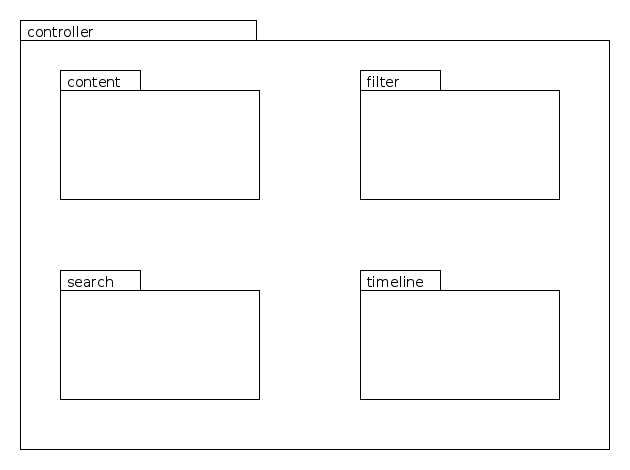
\includegraphics[width=10cm]{package/controller.png}
			\label{gfx:package:controller}
			\caption{Diagramma del package \textit{controller}}
		\end{center}
	\end{figure}

	% SECTION
	\section{Package controller.content}
	\label{ch:stage:design:sistema:controller.content}

	% SECTION
	\section{Package controller.filter}
	\label{ch:stage:design:sistema:controller.filter}

	% SECTION
	\section{Package controller.search}
	\label{ch:stage:design:sistema:controller.search}

	% SECTION
	\section{Package controller.timeline}
	\label{ch:stage:design:sistema:controller.timeline}

\end{document}
